\documentclass[12pt, twoside]{article}
% \documentclass[12pt, twoside]{article}
\usepackage[letterpaper, margin=1in, headsep=0.2in]{geometry}
\setlength{\headheight}{0.6in}
%\usepackage[english]{babel}
\usepackage[utf8]{inputenc}
\usepackage{microtype}
\usepackage{amsmath}
\usepackage{amssymb}
%\usepackage{amsfonts}
\usepackage[nomessages]{fp} %\FPeval{\var-name}{2*sin(pi/6)}
\usepackage{siunitx} %units in math. eg 20\milli\meter
\usepackage{yhmath} % for arcs, overparenth command
\usepackage{tikz} %graphics
\usetikzlibrary{quotes, angles, arrows, arrows.meta}
\usepackage{graphicx} %consider setting \graphicspath{{images/}}
\usepackage{parskip} %no paragraph indent
\usepackage{enumitem}
\usepackage{multicol}
\usepackage{venndiagram}

\usepackage{fancyhdr}
\pagestyle{fancy}
\fancyhf{}
\renewcommand{\headrulewidth}{0pt} % disable the underline of the header
\raggedbottom
\hfuzz=2mm %suppresses overfull box warnings

\usepackage{hyperref}
\usepackage{siunitx}

\title{IB Mathematics}
\author{Chris Huson}
\date{May 2024}

%\fancyhead[LE]{\thepage}
\fancyhead[RO]{\thepage \\ Name: \hspace{1cm} \,\\}
\fancyhead[LO]{BECA/Huson/Algebra II: Regents Prep \\* 13 May 2024}

\begin{document}

\subsubsection*{Practice Regents problems \#11}
AII-F.BF.6 Represent and evaluate the sum of a finite arithmetic
or finite geometric series, using summation (sigma) notation. For geometric series:
$$\sum_{k=1}^{n} a_k = a_1 + a_2 + \ldots + a_n = a_1 \left( \frac{1-r^n}{1-r} \right)$$

\begin{enumerate}
\item Given the sequence $76 \frac{1}{2}$, 51, 34, $22 \frac{2}{3}$ $\ldots$
    %$\frac{3}{2}$, 3, $\frac{9}{2}$, 6, $\ldots$
\begin{enumerate}[itemsep=2cm]
    \item Determine whether the sequence is arithmetic or geometric, then find the common difference $d$ or the common ratio $r$.
    \item Write a recursive formula for the sequence.
    \item Write an explicit formula for the sequence.
    \item Find the sum of the first 8 terms the sequence rounded to the \emph{nearest hundredth}.
\end{enumerate} \vspace{3cm}

\item Simplify each expression. 
\begin{multicols}{2}
    \begin{enumerate}
        \item $\sqrt[3]{64x^9}$
        \item $\displaystyle \frac{10\sqrt[4]{a^{6}}}{5\sqrt{a^{2}}}$
    \end{enumerate}
\end{multicols}
\vspace{3cm}

\newpage
AII-F.LE.2: Construct a linear or exponential function symbolically given: a graph, a description of the relationship, or two input-output pairs (include reading these from a table).

\item Given the quartic function $f(x) = a(x-1)(x-2)^2(x+3)$, graphed below.
\begin{enumerate}[itemsep=1cm]
    \item Is the leading coefficient $a$ positive or negative?
    \item Write down the order of the function.
    \item Over the interval $-1 < x < 0$, is the function increasing, decreasing, or constant? (make sure your answer is consistent with your answer to (a))
    \item Find the average rate of change of the function over the interval from point $A$ to point $B$. \vspace{2cm}
\end{enumerate}
\begin{center}
    \begin{tikzpicture}[scale=0.5]
        \draw[lightgray,very thin] (-10,-9) grid (10,9);
        \draw [thick,<->] (-10.5,0)--(10.5,0) node [right] {$x$};
        \draw [thick,<->] (0,-9.5)--(0,9.5) node [above] {$f(x)$};
        \draw [thick,<->] plot[smooth, domain=-3.3:2.7] (\x, {-0.5*(\x-2)*(\x-2)*(\x+3)*(\x+1)});
        \fill (-1,0) circle[radius=0.15] node [above right] {$A(-1,0)$};
        \fill (0,-6) circle[radius=0.15] node [below right] {$B(0,-6)$};
    \end{tikzpicture}
    \end{center}

\newpage 
\item Go through the steps to factor by grouping $f(x) = x^3+2x^2-x-2$
\begin{enumerate}[itemsep=1cm]
    \item Use your calculator to find the zeros of the function.
    \item Write down the factors of the function.
    \item Write the final row and complete the grouping step by filling in the blanks.
    \begin{align*}
        f(x) &= x^3+2x^2-x-2 \\[0.5cm]
             &= (x^3+2x^2)-(x+2) \\[0.5cm]
             &= \underline{\hspace{1cm}}\;(x+2) - \underline{\hspace{1cm}}\;(x+2) \\[0.5cm]
             &= (x^2-1)(x+2) \\[0.5cm]
             &=
        \end{align*}
\end{enumerate}

\item Go through the steps to factor by grouping $f(x) = x^3+3x^2-4x-12$

\end{enumerate}
\end{document}